\section{感知部分}


\begin{frame}{感知部分}
    \begin{itemize}
        \item 输入:传感数据
        \item 输出:
              \begin{itemize}
                  \item 已探索部分的语义地图
                  \item[+] 预测未探索部分的物体分布
                        \begin{itemize}
                            \item 假设:房间布局的规律
                            \item 全监督训练:更准确、训练更快
                        \end{itemize}
              \end{itemize}
    \end{itemize}
    \note{
        \begin{itemize}
            \item 感知部分负责接受传感器数据,然后输出已探索的部分的语义地图
            \item 除此之外,我们还在感知部分建立显式的预测模块,它将预测未探索部分的语义分布。因为我们认为房间的布局中存在一定规律,例如许多情况下,厨房和餐厅相邻但远离卫生间,卫生间则可能与卧室相邻。
            \item 相比将其集成在全局决策器中,将其单独处理并使用全监督训练或许能达到更好的效果和训练效率。这是我们的设计相对参考的工作的\textbf{创新点}之一
        \end{itemize}
    }
\end{frame}

\begin{frame}{感知部分总体结构}
    \centering
    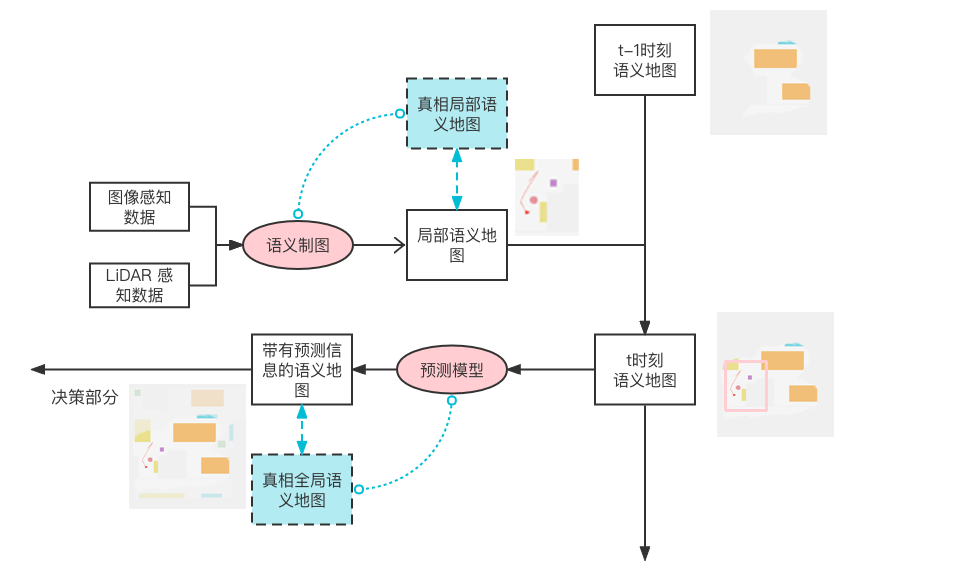
\includegraphics[width=10cm]{assets/perception-example.png}
    \note{
        \begin{itemize}
            \item 感知部分总体上分为两个部分:语义制图和预测模型
            \item 在智能体运行过程中,感知部分将会在每一时刻接收新的传感器数据,在 $t$ 时刻,传感器数据会首先输入语义制图模型,得到关于智能体视野内的局部语义地图。
            \item 得到局部语义地图后,结合上一时刻的已探索语义地图,得到这一时刻更新后的已探索语义地图。
            \item 随后预测模型会对尚未探索的部分进行估计,得到带有预测信息的语义地图,这张地图将会交给决策部分来对长期目标进行规划
        \end{itemize}
    }
\end{frame}

\subsection{语义制图}
\begin{frame}{语义制图模型\cite{objnav}}
    \centering
    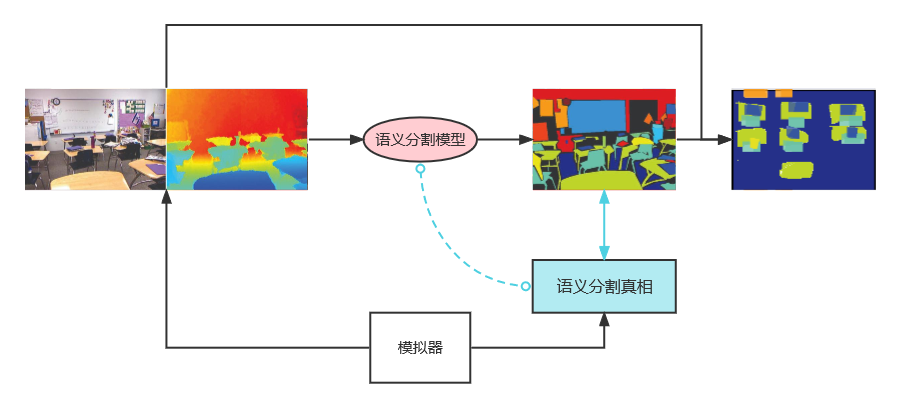
\includegraphics[width=11cm]{assets/semmapping.png}
    \begin{itemize}
        \item 单独训练
        \item 预训练+调优:CMX \cite{cmx}
    \end{itemize}
    \note{
    对于语义制图模型,我们仿照参考文献 [16],使用一个语义分割模型,将传感器的 RGB 和深度信息输入其中,得到语义分割图像。语义分割图像会被用来和模拟器提供的当前视野的语义分割真相来对比,作为模型的监督。

    得到的语义分割会被投射到深度信息给出的点云中,从而确定每一点所属物体的语义。最后从上方观察点云、将语义分布投射到地图上得到局部的语义地图。

    \begin{itemize}
        \item 此模型的输入与智能体的行动方式无关,因此这个模型可以脱离智能体单独训练,也可以采用预训练的大型模型微调。
        \item 我们计划使用多模态语义分割模型 CMX 在场景下 fine-tune 作为语义制图模型。
    \end{itemize}
    }
\end{frame}

\subsection{预测地图}
\begin{frame}{预测模型}
    \centering
    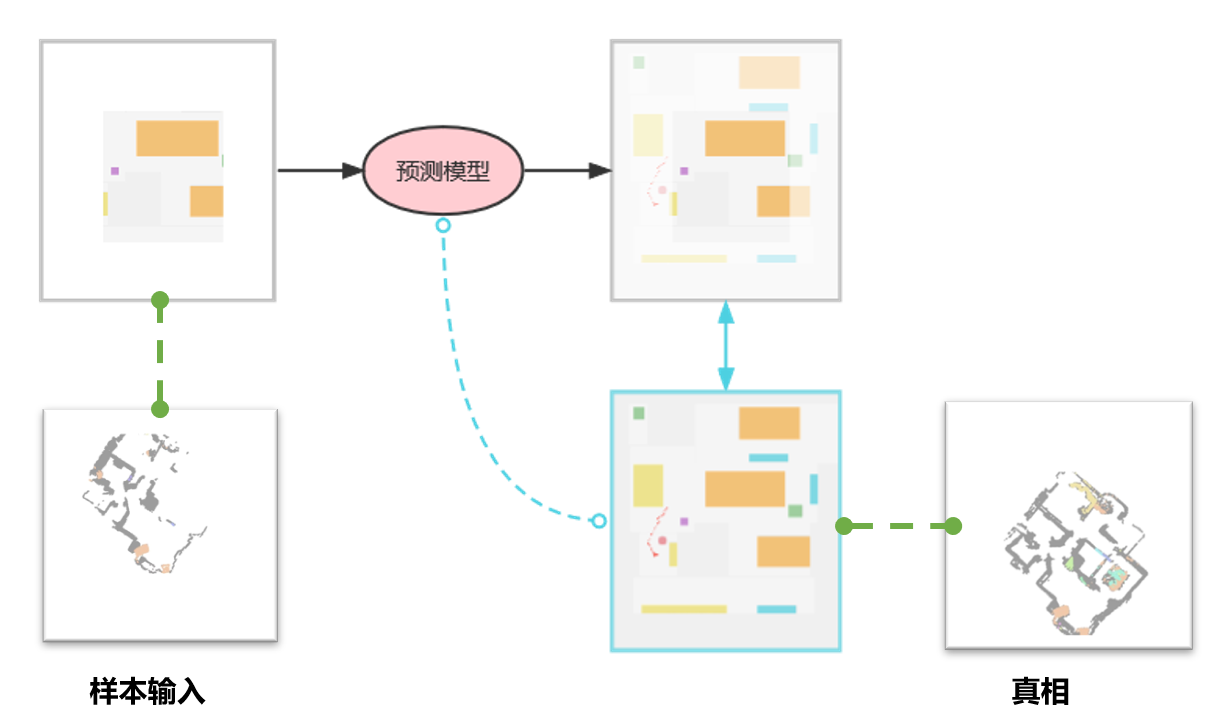
\includegraphics[width=10cm]{assets/predmapping2.png}
    \begin{itemize}
        \item 训练样本的获取:
              \begin{itemize}
                  \item 样本输入:预训练智能体部分观察的语义地图
                  \item 真相:摄像头扫描生成的全局语义地图
              \end{itemize}
    \end{itemize}
    \note{
        \footnotesize
        对于预测模型,我们从模拟器获得真相的全局语义地图作为监督信息,鼓励模型输出的预测结果贴近真实。
        \begin{itemize}
            \item 这一部分处理了语义目标导航任务中,对语义先验的需求。
            \item 由于预测模型的输入——最新时刻的已探索语义地图与智能体的行动方式有关,所以我们令其与智能体同时进行训练。因为我们对预测的显式建模、将其与强化学习部分分离,所以这种训练是通过梯度优化进行的。
            \item 与我们参考的论文 [16] 相比,他们对语义先验的处理方式是将其集成在全局策略器中,然后用强化学习的方法训练。而我们将其使用全监督的方式实现,我们期待这样能让预测结果更好,并且由于使用梯度优化,收敛速度更快。
            \item 监督学习的样本获取:使用自然图像补全方向较新的成果——Diffusion Model所采用的方式。首先需要进行样本数据的收集。输入样本为预训练的智能体在地图上游走收集的部分观察的语义地图;真相为摄像头在地图上扫描生成的完整语义地图。
        \end{itemize}
    }
\end{frame}
